% !Mode:: "TeX:UTF-8" 

\BiChapter{SDN硬件流表可扩展性研究}{the table resource of SDN}


\BiSection{本章引论}{aa}



\BiSection{背景}{aa}

软件定义网络的实时标准为OpenFlow协议,其将网络解耦为控制平面和数据平面。控制平面内可运行网络操作系统,所有传统的网络转发功能都可以由操作系统内应用来完成。网络管理人员只需要开发网络应用即可管理网络内所有设备的行为,通常应用具有标准的通信接口,可支持各类高级语言,且运行环境单一且标准,屏蔽了过去由于设备数量众多导致的开发流程复杂等问题。OpenFlow交换机是支持软件定义网络的标准化设备,负责SDN网络内数据平面内数据包转发操作。OpenFlow交换机支持统一的南向协议,并与控制器通信传递配置信息与数据层状态。

目前高速数据包处理设备性能需求可达数十个Tbps,因此交换机内部需要使用基于硬件的高速缓存(如,TCAM,SRAM等)来进行查表操作。带有掩码功能的查找表(TCAM)是做IP最长前缀查找的高性能核心部件。TCAM具有单周期吞吐的流水线掩码查找能力使得其功能难以由一般存储器代替。但其价格以及能源消耗都较大,基于TCAM的流表容量通常都比较小,且极有溢出的可能。数据包在数据平面中被流表匹配,并得到相应的执行指令,待由后续机构处理。若数据包在流表中没有被成功匹配,则被称作Table-Miss(未匹配)现象。一般未匹配现象的处理方式为丢包,但在OpenFlow协议中支持了reactive处理模式,为后续数据包成功处理,将数据包实时发给控制器,等待控制器处理结果并下发新的可匹配此流的表项。

流表溢出会导致交换机转发性能大幅降低,甚至会导致数据平面与控制器通信报文数量爆炸,给SDN控制器的安全造成隐患\citeup{qsy2018openflow}。网络当中流量变化异常迅速,为减小Table-Miss事件,交换机须能够进行快速流表更新或大容量查找。拥有无限大容量的查找表可以将所有可能出现的流,都预先存储下来。但显然不现实,因此提高流表更新速率成为交换设备的一个硬指标,目前商用交换机的流表更新速度不超过10000条/秒。
基于TCAM的流表删除和添加操作比较复杂,且TCAM有效容量有限,这为设计人员继续增强性能提出了很大难题。

在解决此类问题时,研究人员通常从以下两方面着手:(1)提升流表项数量。当TCAM存储容量固定时,假设宽度为key、深度为depth,二者的乘积恒定。显然如果可以降低流表项宽度值key,可以变相增加流表项数量。在数据中心网络场景下,可以通过重新定义包头域宽度来定义流,无需使用现有过宽的包头域。例如工作\citeup{kannan2013compact}将所有流映射到16bits宽度的匹配域,可增加流表项容量10倍左右,等数据包离开网关时在将原始包头还原。但这种思路仅仅在内网有效,而应对如今更大流量的骨干网,核心网显然无所适从。(2)提高转发设备流表的更新速度。表项替换分为两步,首先控制器选择一条已有表项并删除,之后控制器发送并新增一条表项。一些算法可对TCAM存储空间进行优化合并,表项之间产生依赖。若希望删掉一条逻辑表项,会牵扯大范围的物理存储内容,这增加了修改表项时的操作复杂度,也使得更新表项速度变慢。若流表项剩余空间足够,新增表项可以直接写入空白区域而不去更改已有内容。还可以在运行时检测流表命中频次,提前探测并删除“死流”,为表项争取最大的可用空间。存储分级是一种通用的应对策略,例如使用TCAM+SRAM的双表转发,可大幅度扩展流表数目。考虑到SRAM对带掩码表项资源利用率低,查找速度慢,一般只能将老鼠流存放入SRAM空间,实际应用范围比较窄。

以上这类方法的核心思想是增加表项的原有表项空间,其只能拖延溢出的发生时间,解决思路对缓解流表溢出造成的危害依然无效。本章节针对前文研究不足,提出一种全网流表资源共享机制(Flow Table Sharing,FTS)。其关键解决问题在于流表发生溢出后,如何缓解控制器计算压力,安全通道消息风暴,以及数据平面性能下降的问题。FTS修改了经典Table-Miss处理方式,引入了数据平面与邻居节点组网机制,共同抵抗高突发流量。当流表溢出时对未匹配流量利用本地特殊配置转发策略进行处理,无需立即请求控制器,也不会影响正常运行的流表项。



\BiSection{基于流量特征的问题分析}{aa}

本文通过分析真实流量特征,来证明单纯地依靠增加流表容量无法完全避免流表溢出现象。本文分析ISP服务供应商给出的一段真实数据(新西兰,15分钟,2千万个数据包),发现增大流表容量的确可以减少流表的更新速率。如图\ref{fig:ftsupdate}本文使用最近最少使用(Least Recently Used,LRU)替代算法,当设置流表容量为一万条时,流量变化超过交换机更新极限的情况大约占到10\%。若进一步增大到5万条,约有6\%的流量会引发流表溢出。再将流表容量扩大到25万条,仍有4\%的流量无法得到及时地更新。

\begin{figure}[!ht]
	\centering 
	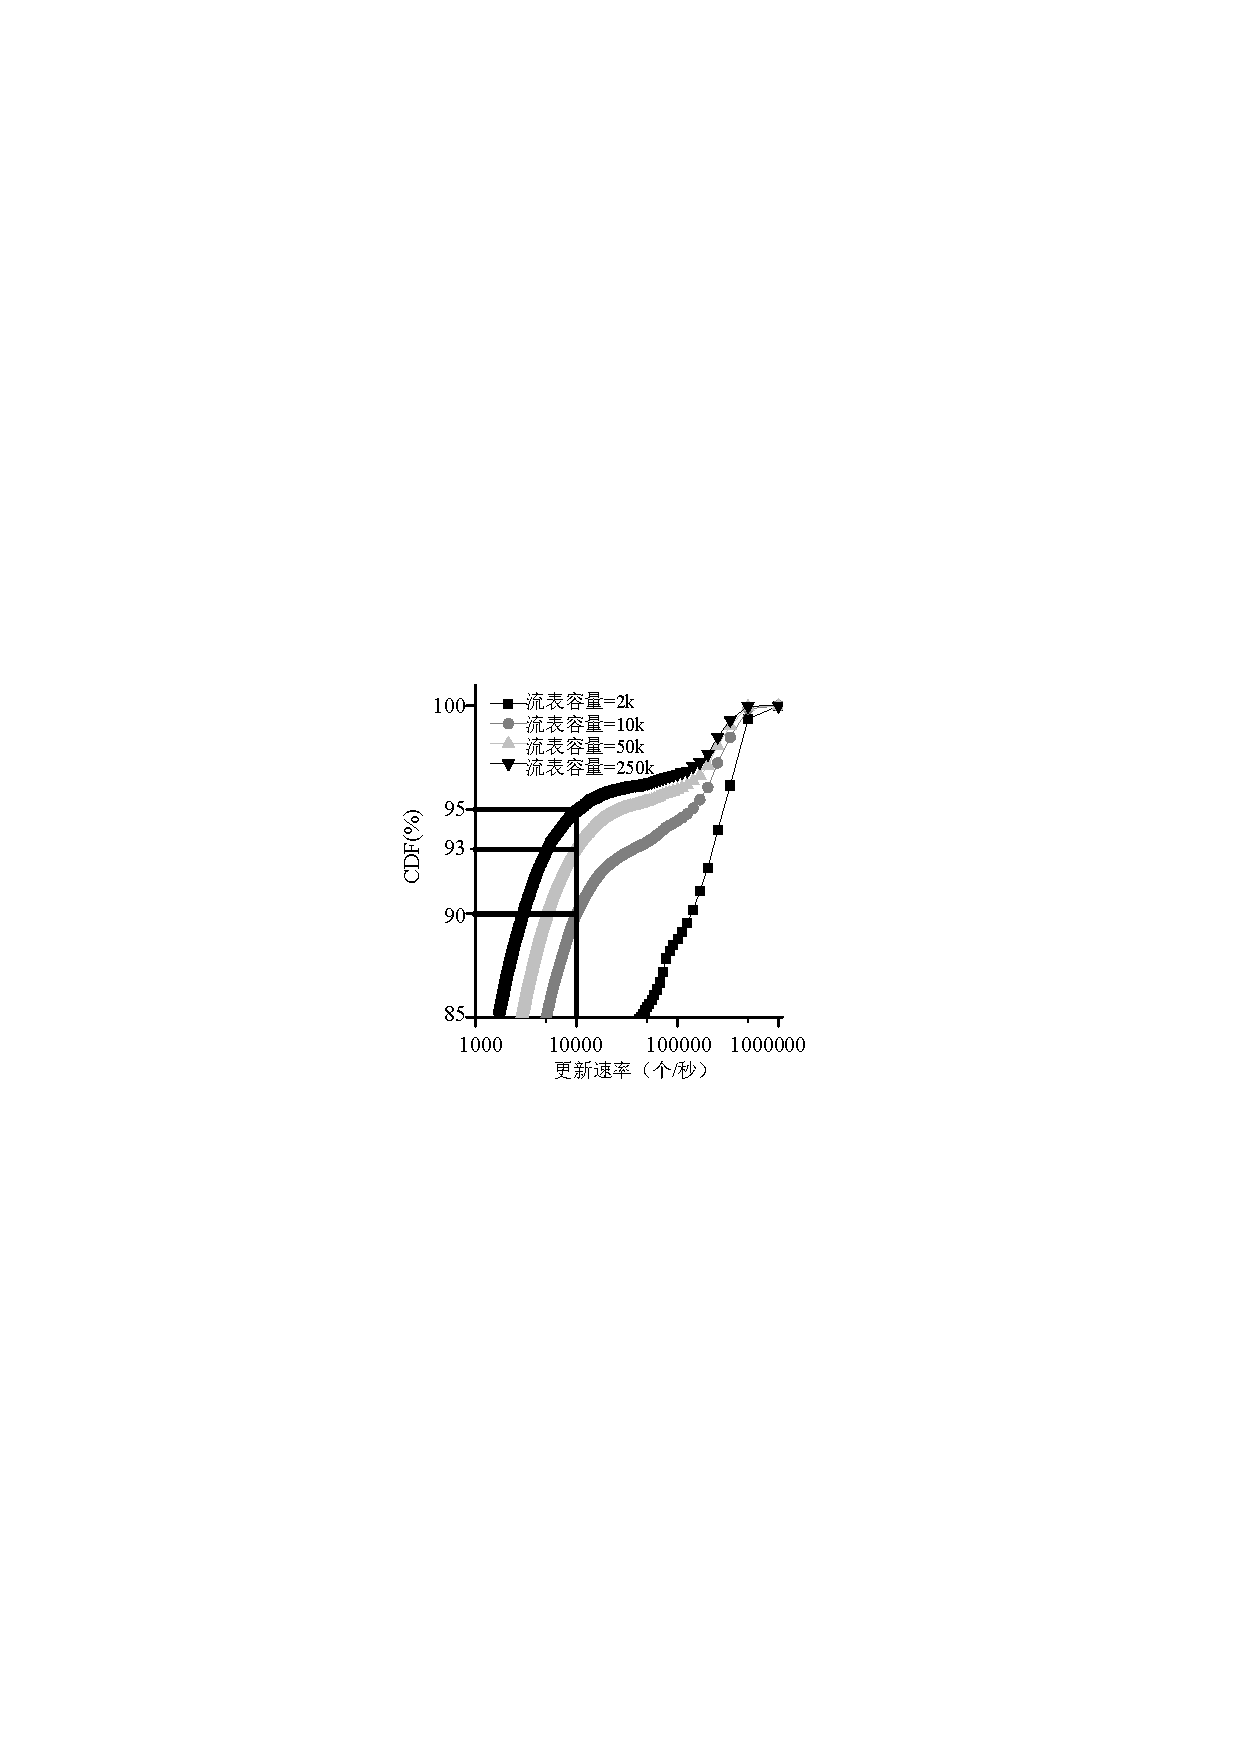
\includegraphics[scale=1]{ftsupdate.pdf}
	\caption{流量更新速率的概率累计分布} \label{fig:ftsupdate}
\end{figure}

根据Openf协议,流表最大支持45个域(144Bytes),流表资源消耗量大的情况在OpenFlow交换机中尤为凸显。面对上述问题,为使SDN的技术优势在广域网间应用,业界不得不使用以及购买性能更强价格更昂贵的交换机。在实际应用中,若交换机流表资源不足,对于最终无法更新的流,交换机会将他们按照Table-Miss策略处理。目前的控制策略大都会以Packet-In消息的方式上报给控制器。若Packet-In消息数目过多,会引起安全通道传输阻塞以及引发控制器处理阻塞,不但会引发控制器安全问题,且影响到其他服务,会加剧数据平面转发效率下降。

\BiSubsection{流量细粒度趋势}{aa}

SDN的核心功能抽象为控制平面向数据平面安装流表项,OpenFlow交换机对数据包的处理过程遵照流表项内容进行转发。基于TCAM的查找表具有高速,流聚合等优良特性,已经广泛使用在交换机中。然而TCAM芯片设计复杂,电路面积巨大,价格高昂(2500人民币/Mbits),功耗大(15瓦/Mbits)。因而交换机无法存储全部流量信息。

如今网络已不局限于best-effort服务理念,服务提供商和内容分发希望流量有区分地进行服务,以提供不同场景不同服务价格,赚取差异化后的最大利益。此外数据中心和蓬勃发展的虚拟云主机市场也对网络流量细粒度管理提出更多需求。尽管OpenFlow协议下流表资源消耗量更大,但市场依然期待让用户得到SDN有利技术。越来越多的实例也展示了SDN技术的强大魅力以及逐步扩大的影响范围。如何应对大规模部署后日益匮乏的流表项资源,以及解决流表溢出导致的性能极端下降,并且如何高效地利用全网有限资源是亟需解决的问题,也是本章探讨的主要内容。


\BiSubsection{问题分析}{aa}

SDN架构使得控制平面与数据平面在物理上分离,控制器与交换机之间通过专用线路建立连接,通常专用线路称作“安全通道”(Secure Channel)。数据平面的配置内容会直接影响到网络的行为,因此对于交换机的配置需要确保严格的安全性。OpenFlow协议利用各类消息定义为应用程序接口,数据和功能打包为数据包在安全通道内传递。SDN对网络的控制因为安全通道传输开销,导致系统控制延迟大于传统网络。研究人员面对了两个源自于SDN架构的挑战:(1)控制平面---消息数量庞大,控制器一般较为复杂、性能需求极高;(2)数据平面---流表空间有限,流表溢出易造成性能大幅下降。

第一类问题,研究人员已经提出了分布式多控制器原理,专用子控制器,提升控制平面的性能方法。本文主要针对第二类问题,即对数据平面可扩展性问题进行研究,分析其可能造成的严重后果。目前OpenFlow交换机有两种实现架构,第一是软件交换机,第二是基于硬件的交换机。二者各有优势,软件交换机通常部署在服务器虚拟机环境内,软件交换机的流表项大多存储于内存空间。服务器内存空间资源通常比较丰富(多达上百GB),足以保存足够多的规则,拥有资源冗余度。软件交换机应用范围有限,主要适用于交换吞吐较低的场景(10Gbps以内)。可将流量较小,流数目丰富的老鼠流交由软件交换机处理。但对于高性能场景(大于1Tbps),依然须使用基于硬件的OpenFlow交换机。

对网络领域进行行为分析,一般使用泊松过程。

\begin{theorem}%[Riesz 表示定理]
	假设数据包的到达服从参数为$\lambda$的泊松过程,$ Flow\_number(T) $为流数量随时间分布,则必然存在某时刻,使得容量为$C$的流表充满。即存在某时刻$t$使得:
	
	\begin{equation}
	Flow\_number(T) \geq C, \qquad T \in (t,t+\Delta t)
	\end{equation}
	
\end{theorem}


\begin{proof}
	假设交换机中流表容量为C条,数据流的到达模式为具有参数$\lambda$的泊松过程,流的生存时间为服从速率参数$\mu$的指数分布,$N_t$为在$t$时刻流表中的流个数。显然,$N_t$是一个增消过程,若到达强度$\rho>1$,$N_t$将无边界增长。因而需满足:
	
	\begin{equation}
	(\rho=\dfrac{\lambda}{C\mu})<1
	\end{equation}
	
	$N_t$的稳态概率密度分布函数推导如下:
	
	
	
	\begin{align}\label{fts1}
	&\pi_0 = [\sum_{k=0}^{C-1}\dfrac{(C\rho)^k}{k!}+\dfrac{(C\rho)^C}{C!}\cdot\dfrac{1}{1-\rho}]^{-1}  \\
	&\pi_k = \begin{cases}\label{fts2}
	\pi_0\dfrac{(C\rho)^k}{k!}, \qquad 0<k<C \\
	\pi_0\dfrac{\rho^kC^C}{C!}, \qquad C \leq k
	\end{cases}
	\end{align}
	
	其中$\pi_k$代表流表中已经有$k(Flow\_number(T))$个流表项的概率。
	参考爱尔兰公式,流表充满的概率为$ P(C\geq  k) $:
	
	\begin{align}\label{fts3}
	P(C\geq  k) &= P(C,\lambda/\mu) \nonumber \\
	&=\dfrac {\left( \dfrac {\left( C\rho\right)^C}{C!}\right) \left( \dfrac {1}{1-\rho }\right) }{\sum ^{C-1}_{k=0}\dfrac {\left( C\rho\right) ^{k}}{k!}+\dfrac {\left( C\rho\right) ^{C}}{C!}\cdot\dfrac {1}{1-\rho }} \nonumber  \\
	&=\dfrac {1}{1+\left( 1-\rho \right) \left( \dfrac {C!}{(C\rho)^{C}}\right) \sum ^{C-1}_{k=0}\dfrac {(C\rho)^{k}}{k!}}
	\end{align}	
	
	由公式\ref{fts2}中$ k $超过$ C $时的概率密度函数,以及公式\ref{fts3},显然不论$ \rho $、$ C $、$\mu$取何值,总有概率$ P(C,\lambda/\mu) $ ,使得$ Flow\_number(T) \geq C $。
\end{proof}

\begin{figure}[!ht]
	\centering 
	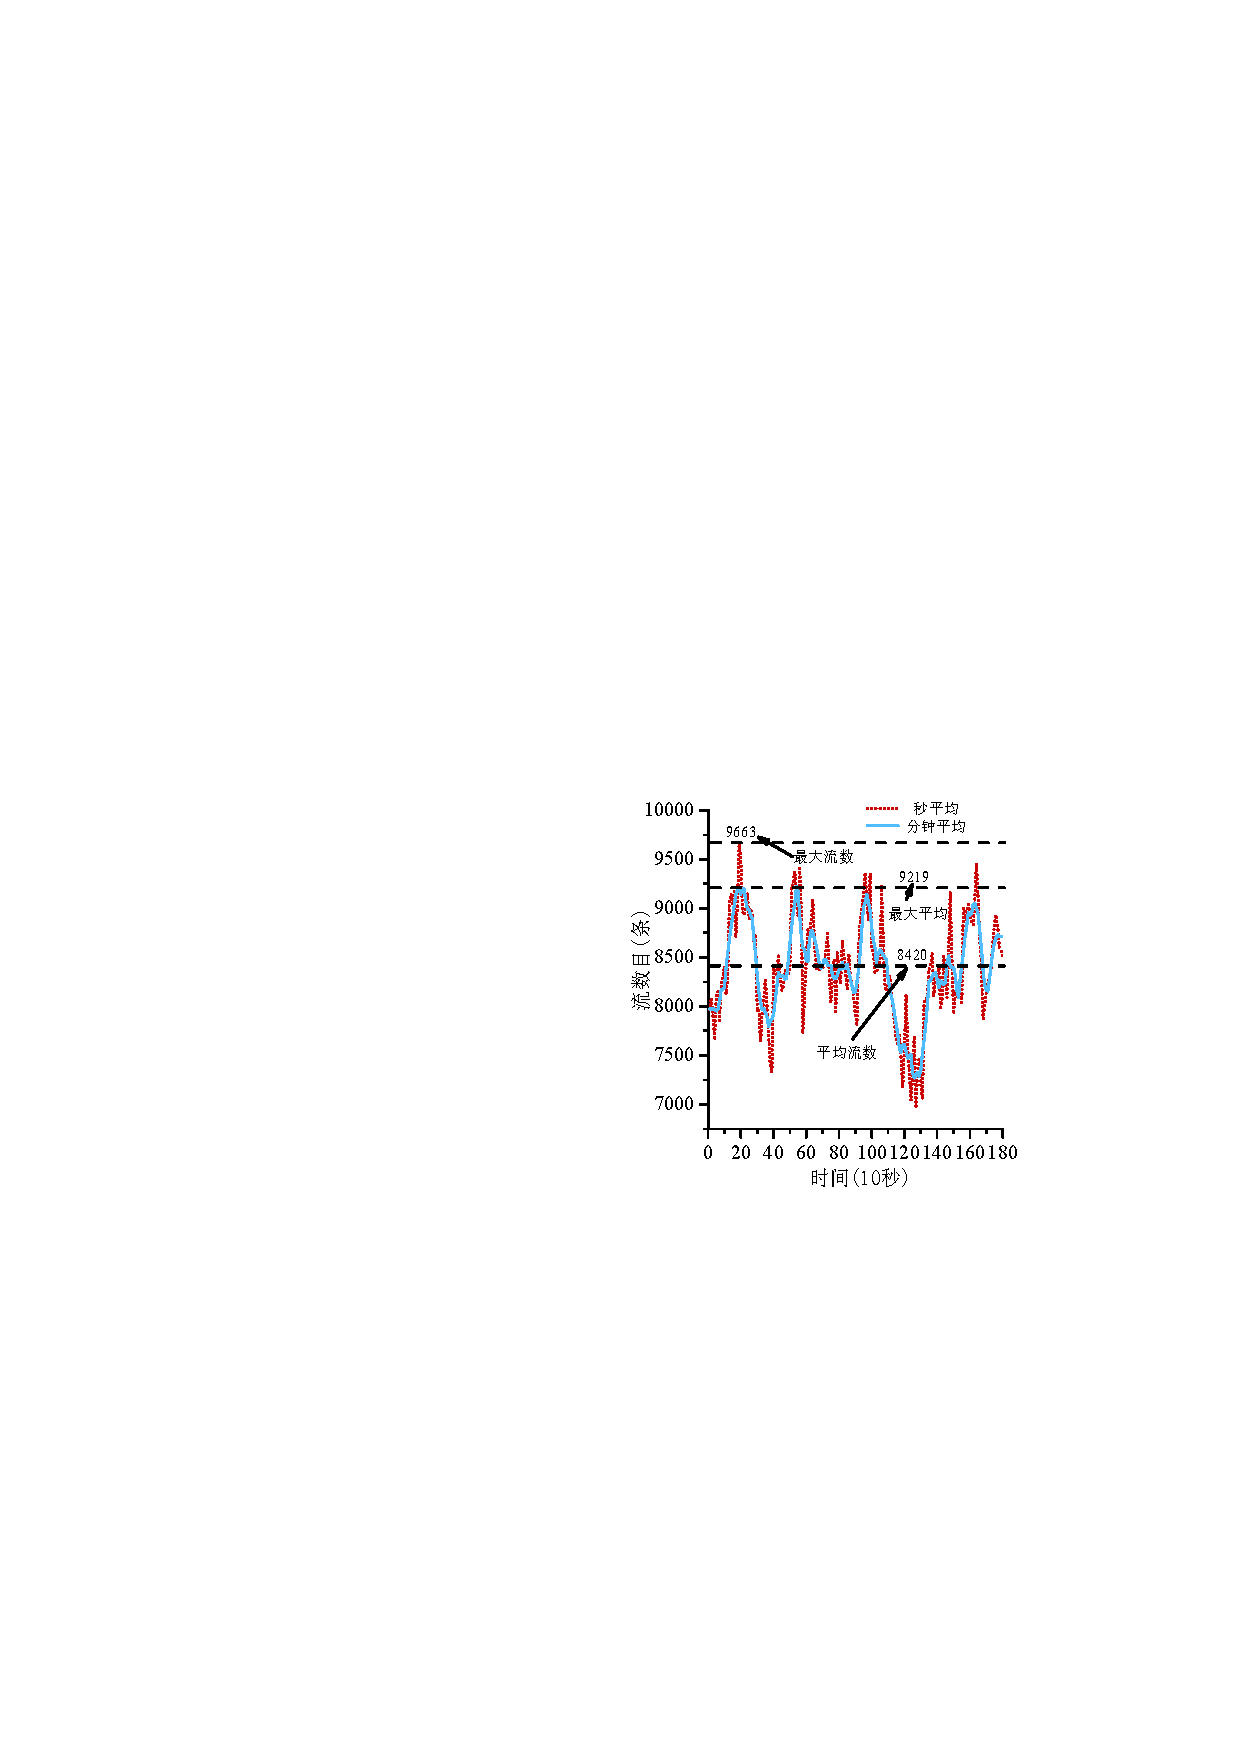
\includegraphics[scale=1]{ftsbigflow.pdf}
	\caption{以10秒为窗口统计流数目} \label{fig:ftsbigflow}
\end{figure}

为得到真实流量特征的统计,本文对广域网(ISP)流量样例进行了分析,并截取如图\ref{fig:ftsbigflow}所示30分钟时间内流数目情况(流分类取前16bit目的IP地址)。可以发现,平均流数目为Avr=8420,假设控制器没分钟对全网流量(削峰填谷)实施调度,则最大流表容量需求为Max\_Avr=9120条。然而在极短暂时刻同时($t+\Delta t$)最多有k=9663条流同时到达交换机。因此可以计算出流数目超过Max\_Avr的概率为8.9\%,剩下91.1\%的时间内,交换机中有7.6\%的流表是空闲的。网络开发人员应根据已有设备的流表资源来决定调度策略的最大精细程度。根据流表使用比例动态调整流表项分布策略是可行的。为保证应用尽用,使经济效益最大化,则有约束条件:

\begin{equation}\label{fts4}
C \leq Max\_Avr \leq k 
\end{equation}

\begin{equation}\label{fts5}
Avr \leq C 
\end{equation}

\ref{fts4}表示容量C若小于最大平均值Max\_Avr有助于提高流表资源平均使用率。公式\ref{fts5}保证流表不可被时时刻刻充满的冗余性条件,因此实际平均使用数目须小于C。在上述两公式的条件下,全局资源中一定有过多的冗余,本文希望减小全网的流表空间浪费率。



%%%%%%%%%%%%%%%%%%%%%%%%%%2020年7月23日22:23:10修改下列文字 qsy

数据平面发生流表溢出的概率始终存在,下面分析流表溢出现象对网络通信服务造成的性能危害。OpenFlow协议规定,当控制器准备对交换机下发流表项时,如果交换机流表已经被装满,交换机会向控制器报告消息<ofp\_error\_msg,OFPFMFC\_TABLE\_FUL-\\
L>,并且交换机端拒绝安装这条流表项。控制器得到错误报告消息后, 可以选择忽视此流,也可以执行流表替换规则:1)忽视此流,造成拒绝服务现象。2)如果控制器采纳此流,则需先删除一条已有流表项,再重新添加此流。但是如果被删除的已有流表项是一条活跃流,继而又造成这条活跃流暂时中断服务。那么会有极大的可能导致数据包传输时延增大,传输带宽变小,甚至丢包。我们将在第五章展示流表溢出后通信效果变差的实验结果。

接下来我们以一个实例来具体分析以上论述:如图3所示,四个节点组成的简单拓扑。每台SDN交换机都与一个SDN控制器相连。假设在某一时刻,S2交换机内流表项被填充满。之后如果另有新流到达,按照现有OpenFlow协议并针对S2交换机分析其操作流程:(1)S2交换机查找表项无匹配结果,并触发Packet-In消息;(2)控制器接收到Table-Miss消息后需要下发新表项,并且控制器计算判断出S2流表已满,选择一条流表项删除;(3)控制器下发新流安装到S2;(4)新流转发建立成功。

值得注意的是控制器删除的那条原有流有可能是一条活动流(active flow),还没有超时,此流后续的数据包会快速到来。但是控制器无法轻易得知:哪条流是最近最长时间没有被匹配的,控制器很难按照最优化的方式删除活动流。当这条流表项被删除后,后续到达的数据包又会被交换机判别为新流,网络控制闭环会重复前面的过程。新流频繁到达将会导致在安全通道内充斥大量重复控制消息数据包,从而耗费了控制器的计算处理资源,占用了安全通道内有限的通信带宽,也降低了交换机的转发效率。
另外也可以假设:控制器发现流表存储已满,不再向交换机内添加新流表项。这种方式保证了已有流量的正常转发,但会导致系统必须放弃对新流的响应。综上所述,本问题最根本的原因是由于流量的起伏波动,流数目暂时越过了交换机容量的上线,导致单个交换机性能下降,进而导致整体网络服务质量下降。


\BiSection{流表共享机制}{aa}

针对之前两章节所遇到的问题,我们提出了一种流表共享机制,该机制设计目标是缓解由于流表溢出而造成的转发能力下降或暂时无法提供服务的现象。流表共享机制从两个关键点进行优化:1)允许流表溢出的交换机转发新流;2)减小重复控制消息的数量。

\BiSubsection{允许流表溢出的交换机转发新流}{aa}

问题:没有建立流表项的流无法被交换机转发转发。经典的<匹配-执行>操作方式,规定数据包在被匹配成功之后才能被处理。当交换机内没有容纳新流的流表空间时,新流匹配表项无法被安装,交换机也无法对新流执行任何操作。然而我们希望当交换机流表溢出时允许转发,这与现行的模式相矛盾。

解决思路:我们为交换机增加了随机转发模式。这与<匹配-执行>不同,随机转发模式将流量随机地转发到邻居节点。这种方式没有宏观的策略指导,转发方向只要不等于入端口方向即可,从而避免路由环路的产生。因而这条本可能被拒绝服务的流,就出现在了邻居节点上。邻居节点与本节点同时发生流表溢出的概率很小,因此这条流会有更大的可能性成功地在邻居节点上建立正确的策略性转发路径。



\BiSubsection{减小重复控制消息的数量}{aa}

问题:新流频繁到来,引发重复的Packet-In消息。在OpenFlow协议下,SDN交换机收到无法匹配的流后,会触发Packet-In消息。Packet-In消息携带了包头信息给控制器,作为控制器判断如何进行包处理的信息依据。若到达的流数量超过了交换机的匹配容量,那么对交换机而言,在当前时段内无法处理的包都可归为新流。这不得不导致携带相同包头信息的控制消息反复在安全通道内传递,降低有效控制信息通信效率。

解决思路:我们将通配转发引入到随机转发模式,通配任何数据包包头。因此对于任意一条额外的新流,都会被匹配,交换机总能保证此数据包被处理,从而不产生重复的Packet-In消息。下一章详细论述FTS结构如何设计与实施。

\BiSection{基于OpenFlow交换机的随机路由策略}{aa}

为抑制在流表溢出时因更新流表而产生重复控制消息,改善因新流没有相应的<匹配-执行>信息而无法获取转发服务的现象,我们提出了<随机转发-流表扩散>的方法。溢出的节点利用邻居节点内空闲的资源,重新建立一条从邻居到目的地的转发路线。

此方法需要在一定的前提下才可正常工作,显然,如果网络中的交换机都随机转发,必然导致数据风暴或者数据包无法抵达目的地。因此我们假设,网络中流表溢出只存在于随机的少量的转发节点中。利用反证法证明:如果网络内大部分结点都发生流表溢出,那么此情境下的网络必处于全面拥塞的状态。根据实际情况,多数时段内网络并不会总出现大规模的全面拥塞。因此网络内流表总是有足够的空余,能满足基本的数据包波动。另外,控制器会实时地根据拥塞情况调整网络流的控制粒度,因而流表项的使用只会趋于一种用尽的动态稳定,再次从宏观角度保障不会有大规模流表溢出的现象发生。


图4是对应于经典SDN网络,采用了缓解机制后的网络结构图。假设交换机S2流表溢出,若此时新流到达,匹配为Table-Miss且交换机不产生Packet-In消息。即在交换机流表溢出后,仅在本地执行离线策略。通过一定的本地计算,快速得到新流的转发动作,从而避免将新流的数据包丢弃。其中的快速算法:随机转发,应满足线速需求。本例中,新流被随机转发到S4中,且之前建立的活动流不会受到本地离线策略的影响,可以继续转发。新流到达S4后,便可在此邻居节点上重新实施路由。下面的两小节将详细说明交换机离线策略的设计以及实现方式。

\BiSubsection{随机路由离线策略设计}{aa}

我们将交换机中的离线随机策略抽象为如下图 5形式:


数据包到达交换机首先查找流表,匹配成功后执行已经设定的处理操作例如,更新计数器,执行指令集等。之后判断流表是处于否溢出状态并且是否需要触发Table-Miss事件:如果没有溢出则直接执行最终的动作集,此处动作集包括但不限于触发Packet-In消息;如果流表溢出,则在交换机本地计算数据包的转发端口。
包含缓解机制的交换机与经典SDN交换机的区别只在增加了判断Table-Miss事件时,交换机是否处于流表溢出状态;以及在交换机离线处理策略中的out\_port端口计算算法的实施。为支持交换机线速转发,以上算法只能在交换机的硬件快速流水线中实施。修改交换机硬件流水线是一件比较困难的事情,然而我们发现流水线内的flow-table,指令集,动作集都可以灵活配置。因此我们只能考虑将此算法与SDN交换机流水线内拥有灵活性的组件耦合起来。
我们将设计的总体流程总结如下:
1.流表匹配。经过流表匹配之后,可以得到packet是否为Table-Miss。 
2.根据metadata以及交换机自身判断提供的流表使用率,判断是否需要本地计算。
3.流水线内的out\_port算法计算数据包的转发端口。
4.执行动作集。
其中必须满足的限制条件:
1.随机转发之后的出端口(out\_port)不能等于入端口(in\_port),否则会产生环路。
2.为满足吞吐率,out\_port随机算法必须简洁高效。
限制条件带来了2个硬件实施上的挑战:
1.实现随机。没有现成的指令集可以完成随机指定动作集。
2.目前OpenFlow协议规定的硬件流水线还没有明确判断流表是否溢出的流水线级。贸然修改SDN交换机流水线则改变了标准的协议,这样会导致交换机可扩展性差的缺点。
为应对以上的挑战,我们选择以组表作为SDN交换机实施随机转发的关键组件。



\BiSubsection{随机路由策略组表方式实现}{aa}

1)OpenFlow组表。

OpenFlow协议规定SDN交换机需包括组表(group-table),组表包含多个动作桶项目。每一个动作桶都包含一个可执行动作集和相关参数。组表类型有:ALL, SELECT, INDIRECT, FAST FAILOVER,四种。我们选择组表的SELECT操作类型。
SELECT:一个数据包只被组内的一个桶执行,这个动作的选取基于交换机的用户选择算法。例如哈希某些用户配置的域,或者简单的循环选择。选择算法的配置和状态不属于OpenFlow协议的范围内。
如图6所示,组表是交换机流水线动作集的一种形式。组表将多个动作集内容通过一定算法联到一起,将给数据包带来更灵活的操作方式。组表包括组表编号字段、组表类型字段、计数器和桶。针对不同的组表类型,桶的执行方式也有所不同。OpenFlow协议规定组表的SELECT算法可以由外部用户自己定义,此选择算法用来选择任意一个可执行的桶,如果当属于一个选定桶的动作集出端口丢失连接,逻辑会自动将桶范围缩小至剩余的可用桶并重新选择。

一些标准的选择算法已经固化在硬件组表内,例如,使用哈希算法来分类用户配置的包头元组,或简单的令牌环。至此,OpenFlow组表解决了上一节提出的两个挑战,即利用随机选择桶算法实现随机,组表天然的又是硬件流水线内的一部分,可以满足线速转发的需求。

下一小节讨论:基于上一节提出的限制条件,我们应该如何设置流表以及组表,即1.出端口不能等于入端口,2.流水线随机算法必须简洁高效。


2)组表桶的设定。

桶内的动作集用来指定数据包转发出口,权重表示执行此桶的概率大小。随机扩散机制要求向邻居转发。那么桶内的动作集中转发出端口(out\_port)的值应该对应自己所有的邻居节点。显然,数据包出端口不能包括入端口,与我们之前的策略相矛盾。在这里我们有两种方式解决:1)结合流表二级匹配,区分并剔除源端口;2)采用额外组表选择算法剔除入端口。
(1)结合流表二级匹配。流表的匹配域为in\_port,设置对应的group\_id = in\_port 的组表。此组表内的桶不包含转发到PORT=in\_port的动作集。之后,由令牌环实现简单高效的随机算法。并且将此流表项配置为最低优先级,保证此流是将要产生Table-Miss事件的。例如,交换机有N个邻居,我们需要添加N条流表项,以及配置N个组表,每个组表内包含N-1个buckets;空间复杂度为O( )。另外,我们考虑流表溢出的判断:其一,我们可以利用控制器判断流表使用情况,一旦溢出,控制器才向交换机内填写N个扩散流表项,但是这会导致较大控制延迟。其二,我们可以利用外部选择算法,在交换机本地判断,控制器可以将N个扩散流表初始化到交换机内。
(2)采用额外组表选择算法。将组表内的selection算法加以扩充,只需要一个组表,组表内动作集包括转发向所有的N个邻居、和1个控制器(CONTROLLER)。如果算法判断交换机流表使用正常没有溢出,直接选择转发向CONTROLLER的桶。在溢出的情况下,选择out\_port时算法同时比较in\_port,随机算法可以用简单令牌环,一旦发现out\_port与in\_port相同则向后跳一个桶执行即可。
总结方法1:空间复杂度大:其中流表O(N)、组表O( );初始化延迟大,但是无需用户大量修改组表内的固有的选择算法。
总结方法2:空间复杂度低:流表O(1),组表O(N),初始化无延迟,但是需要用更换组表内的选择算法。
由于OpenFlow协议对于SELECT算法并没有强加标准,规定SELECT算法是SDN交换机内的可选组件,那么我们更倾向于使用第二种方法,选择定义一种可扩展性强的SELECT算法。算法1列出了选择算法的伪代码。



如图7(a)所示,方框内部表示标准OpenFlow协议规定的组表结构,组表包括了1.组表编号,2.组表类型,3.计数器,4.一个或多个桶,5.随机选择算法,6.外部选择算法。默认随机选择算法是硬件令牌环算法。

如图7(b)所示,外部选择算法从逻辑上,是Table-Miss处理的延伸。这是因为桶内的权重为1,可被作为out-port的候选对象。若某bucket.weight= 0,选择算法会将此bucket对应的action屏蔽。如果所有bucket的weight都为0,此数据包会被丢弃。所以目前Table-Miss的处理方式可以由group方式简单表达。除能扩散算法也很简单,只要将前N个buckets的weight设置为0即可。或者,设置某些bucket的weight为0,即可关闭向对应邻居扩散。至此已完成流表溢出缓解机制的设计介绍,下面我们根据实验结果,对流表共享机制进行评估。





\BiSection{系统评估}{aa}

实验测试分为2个部分,分别是:(1)利用软件仿真平台,对比FTS与优化之前转发性能的优劣。(2)在真实拓扑上测试流表共享机制的实际部署开销。
实验的第一部分转发性能测试使用了软件仿真平台,由于软件仿真在性能上与真实转发设备有一定的差距,因而我们需要讨论软件仿真实验的系统误差估计,主要针对转发时延。计:在流表溢出后的流量总时延为$T_{over\_flow}$,经过FTS优化后的流量时



\BiSection{本章小结}{aa}
